%!TEX root = ../thesis.tex

\section{背景}
一般的に,移動ロボットを目的地まで誘導する制御はナビゲーションと呼ばれ,工場内の巡回や,警備.配送業務などを行う
自律移動ロボットに活用されている.
これらの多くのロボットは,ナビゲーションに
占有格子地図などの事前に作成したメトリックマップを用いている.
% に基づいて
% 自己位置推定,経路計画するナビゲーションにより目的地まで自律移動している.
例として,つくば市内の公道で行われる技術チャレンジである
つくばチャレンジにおいて,
原らが行なった技術調査\cite{hara2019}によると,参加した57チームの中で,50のチームが
メトリックマップに基づくナビゲーションを用いている.
また,これらのチームの多くは,メトリックマップに基づくナビゲーションに
LiDARやIMUなどのセンサ,ホイールエンコーダから算出したオドメトリを利用している.

これらのLiDARやオドメトリ,メトリックマップを基づくナビゲーション
の他に,カメラ画像と深層学習に基づくナビゲーションが研究\cite{kendall2018learning}\cite{sauer2018conditional}されている.
その中で,本研究室の岡田ら\cite{okada2020}\cite{okada2021}は\figref{fig:imi_abs}に示すように
メトリックマップを基づくナビゲーションによる行動を,
視覚を入力とした行動に模倣することで,視覚に基づくナビゲーションを
獲得する手法を提案した(以後,岡田らの従来手法と呼ぶ).
また,提案した手法の有効性を,シミュレータと実ロボットを用いて
検証する実験を行い,視覚に基づいて一定の経路を追従できることを確認している.
この手法の利点として,一般的な模倣学習が人の挙動を模倣するのに対して,
本手法では,メトリックマップに基づくナビゲーションの行動を模倣するため,データセットを収集する手間を省くことが可能という特長がある.
% 学習後はカメラ画像(視覚)のみをセンサ入力として自律移動が可能なことが挙げられる.
% また,メトリックマップに基づくナビゲーションと視覚に基づくナビゲーションを併用し,
% 状況に応じて高い信頼性が見込まれる方を選択することで,経路追従を継続できる可能性が高まる.

岡田らの従来手法では,経路を追従する行動の獲得を目的としていた.
そのため,走行する経路は一定という制限があり,任意の目的地に向けて移動することはできない.
\figref{fig:nav_need}に示す目的地に向けて移動するためには,
環境中の分岐路を検出する機能,分岐路で適切な進行方向を提示する機能,
動的に経路を選択して移動する機能が必要と考えられる.

そこで,本論文では,岡田らの従来手法に対し,
\figref{fig:haru_select}のような分岐路を視覚に基づいて検出する機能,
分岐路で目的地に向けた進行方向を提示する機能,
動的に経路を選択して移動する機能を追加する.
これにより,走行する経路を一定から,任意の目的地に向けた経路へ拡張することで,
視覚に基づいて,経路を追従して目的地へ到達できる可能性がある.
% 目的地までの経路の指示
% また,分岐路といった「通路の特徴」を検出する機能の
% 分岐路で経路が選択できること.
% 目的地までの経路の指示

% カメラ画像
% 実世界では,LiDARやGNSSなどのある特定のセンサが機能しない状況に
% おちいり.ロボットの自律移動を継続することが困難になる場合がある.
% この問題の対処には,複数のセンサを統合して利用する方法や,ロボットに
% ナビゲーション手段自体を複数持たせる(冗長化)する方法が考えられる.

% ナビゲーション手段の冗長化に向けて,
% 本研究室の岡田らは,\ref{fig:imi_abs}に示すように
% 一般的に用いられるLiDARやオドメトリ,
% メトリックマップに基づくナビゲーションの行動を
% 視覚を入力としてend-to-endで模倣学習することで,
% 視覚に基づくナビゲーションを獲得する手法を提案している.
% この手法の特長として,学習のデータセットに利用する行動と
% 学習時にロボットを制御する行動を別々にして扱うことで
% ロボットが経路から外れたときでも,常に経路に戻る行動をデータセットに追加できる.
% また実験を通して,視覚に基づいてロボットが学習した経路を周回可能であることが確認した.
% 岡田らはさらに,訓練時に計測したデータの全てをデータセットに加えるのではなく, 学習器の出力
% を監視して, 経路追従できない場所のデータのみ選択してデータセットに追加する手法を追加している.
% これにより,目標角速度のデータセットの偏りを減少し,角の経路でも経路を追従できる可能性が向上することが
% 確認されている.
\vspace{3zh}
\begin{figure}[htbp]
     \centering
      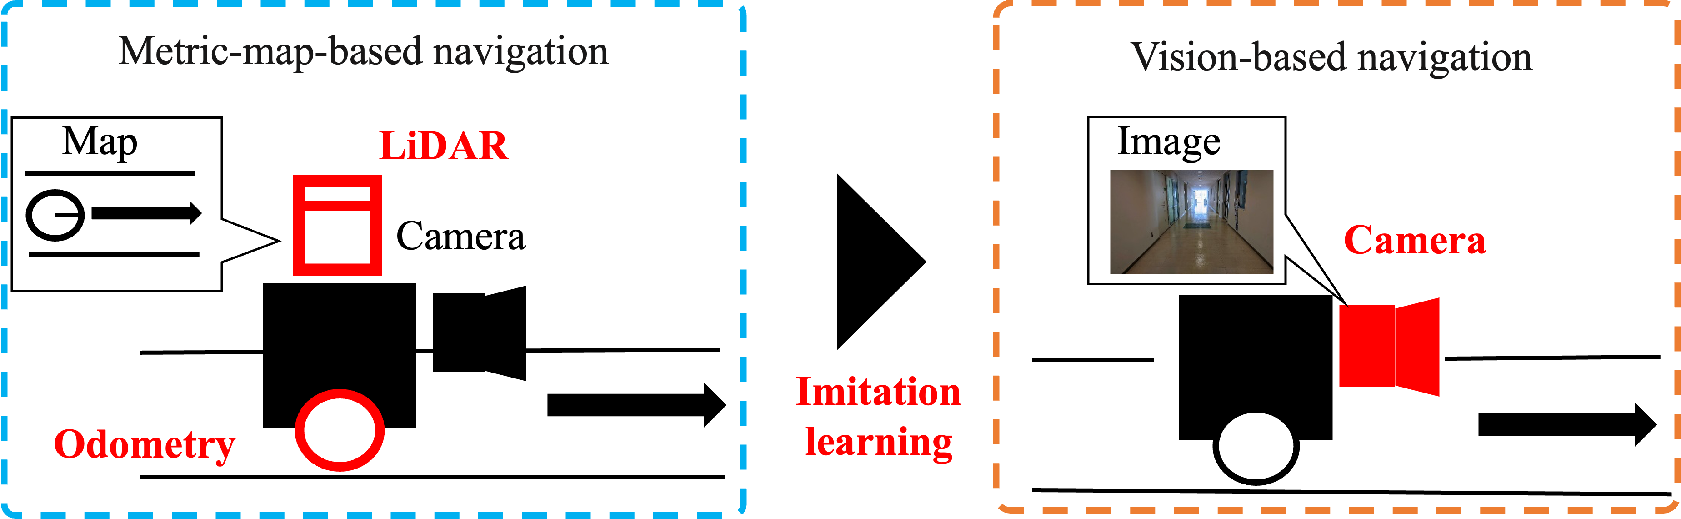
\includegraphics[width=130mm]{images/pdf/imi_abs.pdf}
      \caption{Imitation method of path-tracking behavior}\label{fig:imi_abs}
 \end{figure}


% 春山らは,前述の岡田らの手法に対し,
% 目標とする進行方向の情報(目標方向)を加えることで,
% 視覚に基づくナビゲーションに分岐路で経路を選択して移動する
% 機能を追加している.
% これにより,ロボットは\ref{fig:haru_select}のように
% 指示された方向に移動するように,
% カメラ画像に基づいて経路を移動する
% また,藤原らは,この経路を選択する機能を学習する際に,
% オーバーサンプリングや学習時に積極的に蛇行する手法を取り入れることで,
% 学習時間を短縮する手法を提案している.
% 岡田らの手法では,周回する経路を
\begin{figure}[htbp]
     \centering
      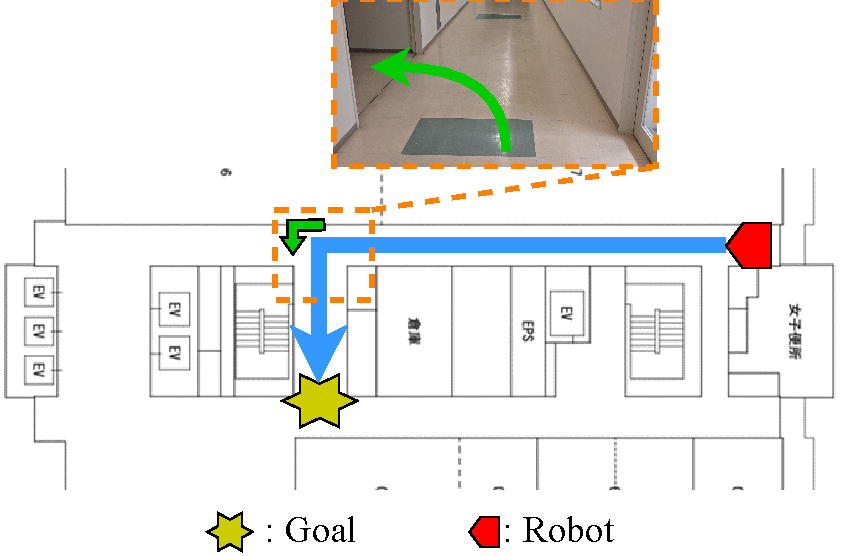
\includegraphics[width=120mm]{images/pdf/nav_need.pdf}
      \caption{Autonomous mobility towards any destination}\label{fig:nav_need}
 \end{figure}
 \begin{figure}[htbp]
     \centering
      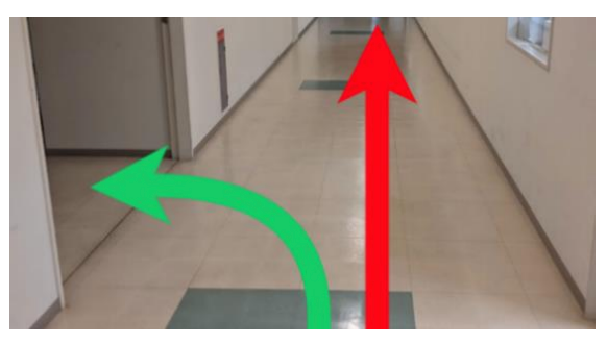
\includegraphics[width=90mm]{images/pdf/branch_path.pdf}
      \caption{Branching paths in the environment and path selection at branching points}\label{fig:haru_select}
 \end{figure}
% 春山らと藤原らの手法では,目標方向の
% 作成方法は議論の対象としておらず,
% 分岐路における目標方向の生成は,カメラ画像から行っていない.
% つまり,視覚のみで目的まで自律移動することは困難となっていた.
% そこで,本稿では,視覚のみで目的地まで自律移動するために,
% 前述の経路を選択する機能をもつ視覚に基づくナビゲーションに対し,
% 目的の分岐路に到達したかの判定を視覚で行い,目標方向を提示する機能を追加
% を追加する.
% このシステムにより,事前に作成したメトリックマップを必要せずに,
% カメラ画像を入力として目的地まで自律移動できる可能性がある.
\newpage
